%----------------------------------------------------------------
%
%  File    :  survey-animation.tex
%
%  Author  :  Fernando Pulido Ruiz, TU Graz, Austria
% 
%  Created :  01 Dec 2016
% 
%  Changed :  X Dec 2016
% 
%----------------------------------------------------------------


\chapter{Animation}

\label{chap:Animation}

{\em"Animation is defined as changing some property over time. On the other hand, motion is the act of moving or the process of being moved. . . .  To put it more simply, all motion is animation, but not all animation is motion."}\citep{head2016designing}

\section{Not Just Motion!} % (fold)
\label{sec:anime_motion}

In animation we change an object’s attribute(s) over time to achieve an objective. As stated by \citet{head2016designing}, animation is much more than adding movement to an object. Movement of an object can be described by a change of its 6 degrees of freedom, them being the coordinates in 3D space and the rotation around the 3D space axises. However an object has usually many more changeable attributes or properties. One could animate color changing and fading, invisibility through transparency, growth with scaling, focus with blurring, etc.

\section{Why Animation in Web UI?} % (fold)
\label{sec:anime_why}

\TODO{Missing: easier navigation, less brain memory load, improve decision making, uder feedback, save screen space}

While writing this survey, with so much animation theory, a hilarious idea was just coming up to mind. Have you ever stopped to think about why some people just seem to be more funny than others? And of course, this happens everyday. Just think about a good joke told by someone with no real humour. It is meaningless. Now, think about the same joke being told by a profesional comedian on TV telling jokes over the weekend. Way more funny, is it not? But the point is, why and how is this be possible?
%In some sense, it has to do with \ldots animation. The fact is that we somehow could be thought as animated objects. We move, we produce sound, and we show our feelings through those moves and sounds. Furthermore, our feelings can even be influenced by how those sounds and moves we see are! So, having made this clear, now it can be better understood the reason of prefering one guy or another one telling the same joke.
It has lots to do with how they speak and how they move! As well of other minor factors. That, I am afraid, is the same as with animation. 

Animation, be it in a cartoon, webpage, app or anywhere else, adds a new level of communication which can be hard to explain , but easy to feel. It creates a special connection between what the message is intended to be, and the receiver. It allows an additional cannel of invisible information to exist, and makes the viewer feel part of the process, and gets his attention grabbed in a practical way. Nowadays, it´s very common to access many sites through different devices. Just think about when trying to know any train timetable. You probably have the app in your Smartphone, but depending on where are you at the moment, you might just google it up and search it through their webpage. Having animation allows sites to connect context and media. A user will just find himself guided throught the process no matter where he is or what device is he using, because of being under some potential animation process. 

But, how do these animations grab people´s atention? There are over twelve basic principles, written by Disney, but two of them are like the foundation of animation, and the rest basically build up from them. Timing and spacing. Timing can be understood as the time length of an action to happen, let’s say the duration of it, while spacing could be explained as the speed changes during one of these actions in an animation. 
\citet{head2016designing} (Chapter 2, page 18) describes their impact with: {\em“Timing and spacing convey the mood, emotion, and reaction of an object.”}

%Both of them act synergistically, transmitting the viewer all of the feelings and advantages listed aboved.

\section{Aim For Invisible Animation} % (fold)
\label{sec:anime_invisible}

In animation, it is very common during the designing process to end up messing things up. As a general rule, as a designer, your one good way to show love to the user is actually not making his or her life harder accomplishing the task at hand. Certainly designers do not hold such ill intentions, but as said before, it is quite easy and happens very often just to have users unnecesarily waiting for an animation to finish or having a hard time finishing a task due to animation. It could be said that the perfect animation is the one which is not noticed. That´s not 100\% accurate, but a good idea in general. 

\vspace{5mm}

{\em“Good interface animations need to be flexible and always feel responsive to a user’s input even if the animation is currently animating.”}\citet{head2016designing} (Chapter 3, page 48)

\vspace{5mm}

Users need feedback to feel themselves listened and understood. Animation can be understood as a bridge which takes the user to a higher quality experience. If an animation doesn’t respect having the user happily informed with feedback, its experience quality will of course drop and so will the trust towards the UI. A user will never feel comfortable in a system which does not take into consideration its input. 

It is also important, that an animation should never be a show-off work. It should be always remembered, that in general, the user interacting with an animation, is probably willing to do or finish something. A UI user is not just laying there waiting for an animation to happen and look at it itself and enjoy it. That could be the aim of animators years ago where they were really telling stories and people were fascinted about it. But times changed, and now the timing requirements are no longer the same as in those days. Study and carefully think about the suitable timing for each animation, because a short amount of milliseconds can be the limit between failing or succeeding. Good timing is more an art than a science \citep{head2016designing}.
%(when talking about a user’s satisfaction, of course). Val Head [2016] smartly points out that good timing is more an art than a science(PARAPHRASING: VAL HEAD’S BOOK, CHAPTER 3, PAGE 52).

\section{Development of animation} % (fold)
\label{sec:anime_dev}

\TODO{Missing part, COPIED JUST THE POINTS FROM SLIDES}

Often problems in development

Usually discussed at the end stages of the project.
Seen just as extra decoration.
Should be part of the design!
When everything is finished, it is "too late" to replan design (animation).
Animation is underestimated in design.

Where to start planning?

Start with planning already in early stages.
Animation can replace a fixed design element.
Add only animation that helps user and does not distract or lowers the UX.
Write about animation also in style guides and documentation.
Understand basic principles of animation (Disney 12 or other) and how they effect the user.
All important information most support accessibility(Animation is visual information).

How to plan?

In early stages storyboard sketching.
During design prototyping prototype also animation (it is part of the design).

\begin{figure}[tp]
\centering
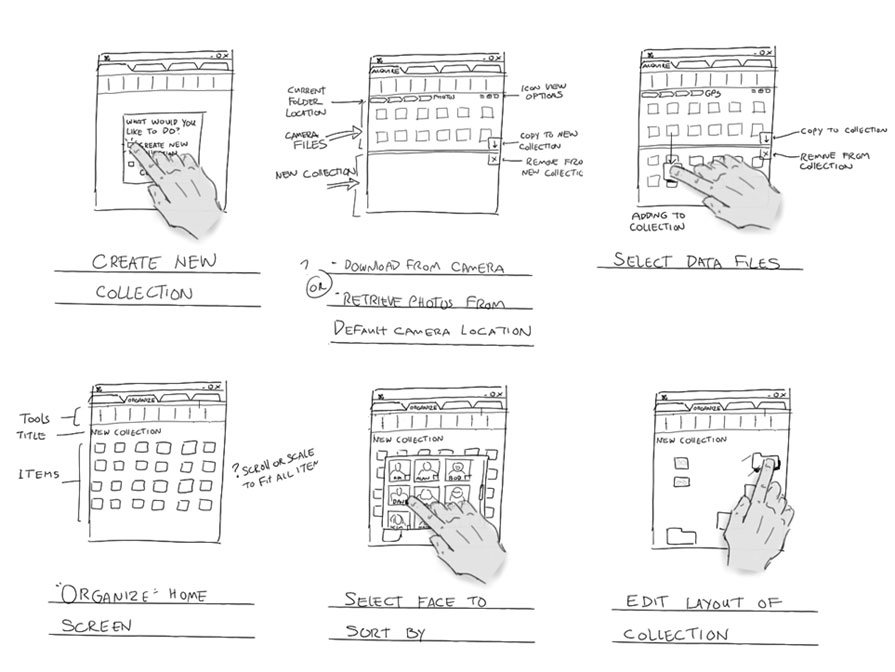
\includegraphics[keepaspectratio,width=\hsize,height=\halfh]
{images/storyboard.jpeg}

\caption[Storyboard Sketching]{
Example of storyboard sketching for drag and drop animation \citep{microsoftStoryboard}.
\imgcredit{Used with permission from Microsoft - Microsoft Copyrighted Content Guidelines}
}
\label{fig:storyboard}
\end{figure}
